\section{Praktická část}

Tato kapitola popisuje knihovnu ExiL, která je výsledkem této práce.
Nejprve popíšu její instalaci a prerekvizity nutné k jejímu používání. Pak v
uživatelské příručce představím její možnosti a typickou strukturu programu,
který ji využívá. Poté v~referenční příručce shrnu všechny možnosti, které
knihovna poskytuje. Nakonec v části věnované implementaci popíšu architekturu
zdrojového kódu knihovny a algoritmus RETE sloužící k efektivnímu vyhodnocování
podmínek pravidel a~zmíním zajímavé části kódu implementující jednotlivá
rozšíření.

\subsection{Common Lisp}
\begin{framed}
\begin{itemize}
  \item základní znalosti lispu nutné pro používání knihovny
  \begin{itemize}
    \item loadování souborů - poté zjednodušit v kapitole o instalaci
    \item package, export, import, shadow
    \item seznam, atom, car, cdr, plist
    \item symbol, klíč
    \item prefixová syntax, S-expressions
    \item funkce, makro
    \item načítání souborů.
    \item quotování (u funkčních alternativ, ale ty se stejně používají spíš z jiného
      kódu, který knihovnu volá - tudíž uživatel evidentně lisp zná)
    \item lexikální prostředí - u vyhodnocení aktivací pravidla
    \item destrukturující makra - tamtéž
    \item výjimky
  \end{itemize}
  \item odkaz na practical common lisp, clhs
\end{itemize}
\end{framed}

\clearpage
%%%%%%%%%%%%%%%%%%%%%%%%%%%%%%%%%%%%%%%%%%%%%%%%%%%%%%%%%%%%%%%%%%%%%%%%%%%%%%%%
\subsection{Instalace}
\subsubsection{Získání zdrojového kódu}
Zdrojový kód knihovny je přiložen k~této diplomové práci a~lze jej také získat
zklonováním\footnote{\url{http://git-scm.com/docs/git-clone}}
gitového\footnote{\url{http://git-scm.com/}} repozitáře na adrese
\verb|git@github.com:Incanus3/ExiL.git|.
Kód knihovny se nachází v podadresáři \verb|src|, ten budu dále nazývat kořenovým
adresářem knihovny či projektu.
%%%%%%%%%%%%%%%%%%%%%%%%%%%%%%%%%%%%%%%%%%%%%%%%%%%%%%%%%%%%%%%%%%%%%%%%%%%%%%%%
\subsubsection{Prerekvizity}
Pro práci s knihovnou ExiL potřebujeme lispový
interpreter\footnote{\url{http://en.wikipedia.org/wiki/Interpreter_(computing)}}
\footnote{lispové interpretery jsou většinou zároveň
kompilátory\footnotemark[6], označením
interpreter tedy budu nazývat obojí},
vývojové prostředí (s interpreterem bychom si ve skutečnosti vystačili, ale
přímá práce s ním není většinou příliš pohodlná) a knihovny umožňující
dávkové načtení celého projektu včetně závislostí.
\footnotetext[6]{\url{http://en.wikipedia.org/wiki/Compiler}}

Knihovnu jsem vyvíjel v prostředí
SLIME\footnote{\url{http://www.common-lisp.net/project/slime/}}, což je plugin
pro textový editor GNU Emacs\footnote{\url{http://www.gnu.org/software/emacs/}}
(poskytující mimo jiné pomůcky pro editaci lispového zdrojového kódu,
REPL\footnote{\url{http://en.wikipedia.org/wiki/Read-eval-print_loop}} a
debugger\footnote{\url{http://en.wikipedia.org/wiki/Debugger}})
s interpreterem SBCL\footnote{\url{http://www.sbcl.org/}} a tuto kombinaci
mohu vřele doporučit. V operačním systému Debian GNU Linux, který jsem pro vývoj
použil, lze Emacs, SLIME i SBCL nainstalovat z výchozího repozitáře a aktivovat
úpravou inicializačního souboru Emacsu, viz
\url{http://www.common-lisp.net/projects/slime/doc/html/Installation.html}.
Prostředí poté můžeme v~Emacsu spustit voláním příkazu \verb|slime|
(\verb|<Alt+X>slime<ENTER>|). Při prvním spuštění se kód prostředí kompiluje, což
může chvíli trvat, pak už se v editoru otevře buffer\footnote{emacs buffer}
s~lispovým REPLem.

Knihovnu jsem testoval také ve vývojovém prostředí
LispWorks\registered\footnote{\url{http://www.lispworks.com/}} Personal Edition
6.1, pro které jsem také vytvořil minimalistické grafické uživatelské rozhraní.
Součástí prostředí LispWorks je i lispový interpret. Prostředí můžeme získat zde
\url{http://www.lispworks.com/downloads/index.html} a nainstalovat podle návodu,
který se zobrazí po vyplnění formuláře.

Pro efektivní načtení knihovny včetně závislostí potřebujeme ještě dvě knihovny:
\begin{itemize}
  \item ASDF\footnote{\url{http://common-lisp.net/project/asdf}} je knihovna
    umožňující snadnou definici struktury projektu a jeho dávkové načtení,
  \item quicklisp\footnote{\url{http://www.quicklisp.org/beta/}} staví na knihovně
    ASDF a umožňuje pohodlně stáhnout a načíst knihovny třetích stran z internetové
    databáze.
\end{itemize}
Knihovna ASDF je součástí instalace interpreteru SBCL i prostředí LispWorks.
Knihovnu quicklisp jsem k projektu přiložil a pokud není součástí prostředí, je
automaticky načtena před načtením ExiLu.
%%%%%%%%%%%%%%%%%%%%%%%%%%%%%%%%%%%%%%%%%%%%%%%%%%%%%%%%%%%%%%%%%%%%%%%%%%%%%%%%
\subsubsection{Načtení knihovny}
V prostředí SLIME načteme knihovnu načtením souboru \verb|load.lisp| z kořenového
adresáře knihovny, tedy zadáním \cl|(load "cesta/k/projektu/src/load.lisp")|
v~REPLu). Tento soubor nejprve načte knihovnu \verb|quicklisp|, je-li potřeba,
a s její pomocí poté načte celý projekt ExiL včetně závislostí. Nakonec soubor
definuje výchozí prostředí, viz sekce \ref{multiple environments}

V prostředí LispWorks načítání pomocí knihovny \verb|quicklisp| nefunguje správně,
knihovnu je proto třeba načítat načtením souboru \verb|load-manual.lisp| (opět
z kořenového adresáře projektu). Načíst můžeme opět voláním \verb|load| v~REPLu,
nebo vybráním položky \verb|Load...| v nabídce \verb|File| menu libovolného okna
prostředí.

Všechna makra a funkce, které knihovna definuje pro přímé volání uživatelem jsou
\emph{exportována} z \emph{package} \verb|exil|. Před interakcí s knihovnou je
tedy třeba vstoupit do package \verb|exil-user|, který symboly z~package
\verb|exil| \emph{importuje}. Symboly z~package je také možno importovat do
existujícího package takto:
\begin{minted}{cl}
  (defpackage :my-package
    (:documentation "user-defined package")
    (:use :common-lisp :exil)
    (:shadowing-import-from :exil :assert :step))
\end{minted}
Package \verb|exil| exportuje několik symbolů, které již v package
\verb|common-lisp| existují. Ty je třeba \emph{zastínit}, jak je vidět z ukázky.

\clearpage
%%%%%%%%%%%%%%%%%%%%%%%%%%%%%%%%%%%%%%%%%%%%%%%%%%%%%%%%%%%%%%%%%%%%%%%%%%%%%%%%
\subsection{Uživatelská příručka}
\subsubsection{Základní pojmy}
\begin{framed}
  \begin{itemize}
    \item TODO: v teoretické části uvést pojmy znovu s citacemi
    \item TODO: production memory v exilu splývá s pravidly znalostní báze - na
      příhodném místě uvést, že v teorii a některých systémech se rozlišuje
  \end{itemize}
\end{framed}

Nyní stručně zadefinuji základní pojmy, nutné pro pochopení fungování knihovny
ExiL a práci s ní. Význam pojmů bude jasnější, jakmile si je ukážeme na
příkladech. K těmto pojmům se posléze vrátím i~v~teoretické části textu
a~jejich popis rozšířím o další souvislosti.

První dva pojmy staví na pojmu znalost, který chápeme intuitivně a nebudu se jej
ani snažit definovat, nikoli na následujícím pojmu znalosti, jak ji chápeme
v~ExiLu (v takovém případě by byla definice cyklická).

Pojem expertního systému zatím chápejme tak, jak jsem jej představil v úvodu
práce. V praktické části rozeberu pojem v potřebné šíři.
\begin{description}[leftmargin=6cm,style=sameline,align=right,labelsep=0.5cm]
  % \item[problémová doména] množina pojmů relevantních pro řešení určité skupiny
  %   problémů
  \item[fakt] elementární statická znalost - tvrzení
  \item[(odvozovací) pravidlo] elementární odvozovací znalost - pokud víme, že
    (ne)platí nějaká tvrzení, můžeme odvodit, že platí i~nějaká další
  \item[znalost (v ExiLu)] množina faktů a pravidel
  \item[znalostní báze] výchozí znalost expertního systému
  \item[pracovní paměť] aktuální množina faktů
  % \item[production memory] aktuální množina pravidel
  \item[inference] odvozování - postupná aplikace odvozovacích pravidel
\end{description}
Pojem \emph{pracovní paměť} není příliš intuitivní. Jde o doslovný překlad
v~literatuře užívaného pojmu \emph{working memory}, kterým je označována množina
faktů (tvrzení), které expertní systém v danou chvíli považuje za platné. Nejde
tedy ve skutečnosti o paměť, nýbrž o obsah pomyslné paměti. Pojem pracovní
množina faktů by byl jistě výstižnější, bohužel ale také značně těžkopádný.

%%%%%%%%%%%%%%%%%%%%%%%%%%%%%%%%%%%%%%%%%%%%%%%%%%%%%%%%%%%%%%%%%%%%%%%%%%%%%%%%
\subsubsection{Struktura programu}

\begin{listing}[h]
\caption{Základní struktura exilového programu}
\label{typical structure}
\begin{clcode}
;;; definition of knowledge base
;; facts
(deffacts world
  (in box A)
  (in robot B)
  (goal move box A B))

;; inference rules
(defrule move-robot
  (goal move ?object ?from ?to)
  (in ?object ?from)
  (- in robot ?from)
  (in robot ?z)
  =>
  (retract (in robot ?z))
  (assert (in robot ?from)))

(defrule move-object
  (goal move ?object ?from ?to)
  ?rob-pos <- (in robot ?from)
  ?obj-pos <- (in ?object ?from)
  =>
  (retract ?rob-pos)
  (retract ?obj-pos)
  (assert (in robot ?to))
  (assert (in ?object ?to)))

(defrule stop
  (goal move ?object ?from ?to)
  (in ?object ?to)
  =>
  (halt))

;;; initialization of working memory
(reset)

;;; inference execution
(run)
\end{clcode}
\end{listing}

Příklad \ref{typical structure} na straně \pageref{typical structure} ukazuje
minimální strukturu programu nad knihovnou ExiL (dále exilový program). První
část programu tvoří definice znalostní báze. Ta sestává z definic faktů, ze
kterých expertní systém vychází a definic odvozovacích pravidel, jež jsou
následně aplikována při inferenci.

Definice faktů jsou uspořádány do skupin označených názvem (v tomto případě
\verb|world|). V ukázkovém programu si snadno vystačíme s jednou skupinou faktů,
v reálných programech bude ale těchto skupin většinou více. Tato organizace
umožňuje snadnou redefinici, případně odebrání, jen některých skupin faktů v
případě potřeby.  Definice skupiny faktů \verb|world| v příkladu přidává do
znalostní báze informaci o~počáteční pozici robota, krabice a~o~našem záměru
přesunout krabici z~pozice \verb|A| na pozici \verb|B|.

Následuje definice odvozovacích pravidel. Definice každého pravidla sestává
z~množiny podmínek, tedy předpokladů pro jeho splnění (a následnou aktivaci),
a~množiny důsledků, tedy libovolných lispových lispových výrazů, které jsou při
aktivaci pravidla vyhodnoceny.  Tyto dvě množiny jsou od sebe odděleny
\emph{symbolem}~\verb|=>|.

Podmínky odvozovacích pravidel jsou ve formě vzorů (\emph{pattern}). Struktura
vzorů je stejná jako struktura faktů (viz sekce \ref{knowledge base
definition}), ale narozdíl od nich mohou obsahovat proměnné (symboly začínající
otazníkem).  Při vyhodnocování podmínek pravidla je zajišťěna
konzistence vazeb těchto proměnných a výskyty všech proměnných v~důsledcích
pravidla jsou při jeho aktivaci nahrazeny jejich vazbami. Detaily viz sekce
\ref{inference}

Důsledky pravidel typicky obsahují příkazy pro modifikaci pracovní paměti (viz
sekce \ref{modifikace}), tedy přidání (\verb|assert|), odebrání (\verb|retract|),
či úpravů (\verb|modify|) faktů v ní. Nemůsí
tomu tak ale být vždycky - důsledkem aktivace pravidla může být např. vypsání
výstupu, logování, zápis souboru, ale také např. ovládání externího systému.

Náš ukázkový příklad definuje tři odvozovací pravidla. Pravidlo
\verb|move-robot| je aktivováno, pokud chceme přesunout nějaký objekt z pozice
\verb|?from| na pozici \verb|?to|, objekt se nachází v pozici \verb|?from|
a~robot nikoli (třetí podmínka je negovaná, viz sekce \ref{knowledge base
definition}). Poslední podmínka slouží pouze k navázání původní pozice robota.
Při aktivaci pravidla je v pracovní paměti nahrazena informace o~původní pozici
robota pozicí \verb|?from|. Robot se tedy nyní nachází na stejné pozici, jako
kýžený objekt.

Podmínky pravidla \verb|move-object| vyžadují, aby byl jak robot, tak objekt
určený k přesunu, na pozici \verb|?from|. Při jeho aktivaci je robot i s objektem
přesunut na pozici \verb|?to| nahrazením faktů o původních pozicích novými,
podobně jako v prvním pravidle. Definice pravidla obsahuje speciální notaci (s
použitím operátoru \verb|<-|), jejímž účelem je navázání celého faktu na
proměnnou. Ten pak můžeme v důsledcích snadno ostranit z pracovní paměti.

Poslední pravidlo slouží k zastavení inference, pokud se již objekt nachází na
zamýšlené pozici. Inference je zde zastavena explicitním voláním \verb|(halt)|.
Druhou možností by bylo odstranit z pracovní paměti fakt definující cíl, neboť v
takovou chvíli nemůže být žádné další pravidlo splňeno.

Jakmile je znalostní báze nadefinována, můžeme z ní inicializovat pracovní
paměť. To provedeme voláním \verb|(reset)|, které (po případném vyčištění
původních faktů) přidá do pracovní paměti fakta ve všech definovaných skupinách.

Poslední nutnou fází exilového programu je spuštění inference. To můžeme udělat
nejjednodušeji voláním \verb|(run)|. Inferenční mechanismus poté postupně
vyhodnocuje, která odvozovací pravidla mají splněné všechny podmínky, v každém
kroku z nich jedno vybere a aktivuje jej. Detaily viz sekce \ref{inference}

Výstup programu je následující:
\begin{minted}{cl}
==> (IN ROBOT B)
==> (IN BOX A)
==> (GOAL MOVE BOX A B)
Firing MOVE-ROBOT
<== (IN ROBOT B)
==> (IN ROBOT A)
Firing MOVE-OBJECT
<== (IN ROBOT A)
<== (IN BOX A)
==> (IN ROBOT B)
==> (IN BOX B)
Firing STOP
Halting
\end{minted}
Řádky začínající symbolem \verb|==>| označují fakty přibyvší do pracovní paměti,
řádky začínající \verb|<==| fakty z paměti odstraněné. Tento výstup obdržíme
pouze pokud zapneme sledování faktů voláním \verb|(watch facts)| (viz sekce
\ref{inference tracing}). První tři fakty přibydou do pracovní paměti při
vyhodnocení volání \verb|(reset)|, další pak spolu s postupnou aplikací
odvozovacích pravidel. Dotážeme-li se po skončení inference na seznam faktů v
pracovní paměti voláním \verb|(facts)|, obdržíme výstup
\cl|((GOAL MOVE BOX A B) (IN ROBOT B) (IN BOX B)).|
Robot i krabice jsou tedy na cílové pozici.

Kód exilového programu má deklarativní charakter. Nikde jsme nemuseli
specifikovat, jakou posloupností akcí má systém k výsledku dospět. To nás ovšem
nezbavuje nutnosti chápat fungování inferenčního mechanismu ExiLu. Nebudeme-li
při konstrukci programu opatrní, může výpočet snadno dospět k neočekávaným
výsledkům, dostat se do slepé větve, či se zacyklit. Tyto problémy jsou často
způsobeny nezamýšlenou interferencí podmínek pravidel s důsledky jiných.

\FloatBarrier

%%%%%%%%%%%%%%%%%%%%%%%%%%%%%%%%%%%%%%%%%%%%%%%%%%%%%%%%%%%%%%%%%%%%%%%%%%%%%%%%
\subsubsection{Definice znalostní báze}
\label{knowledge base definition}
\begin{framed}
  \begin{itemize}
    \item skupiny faktů
    \item pravidla
      \begin{itemize}
        \item podmínky podrobně - patterny, konjunkce, negace
        \item důsledky - typicky modifikace pracovní paměti
      \end{itemize}
    \item queries - fact-groups, rules + finders
    \item přesunout přílišné podrobnosti do referenční příručky
  \end{itemize}
\end{framed}

ExiL, stejně jako CLIPS, rozlišuje dva typy faktů - jednoduché (\emph{simple,
ordered}) a strukturované (\emph{templated}). Stuktura jednoduchého faktu je udána
pouze pořadím \emph{atomů}, typickou volbou je např. \verb|objekt-attribut-hodnota|:
\cl|(box color red),| či \verb|relace-<zůčastněné objekty>|: \cl|(in box hall).|

Strukturované fakty mají naproti tomu explicitně pojmenované složky (sloty).
Typicky popisují objekt s množinou atributů: \cl|(box :color red :size small),|
či relaci s jasně danými aktory: \cl|(in :object box :location hall),| kde
\verb|box| a \verb|in| jsou šablony (\emph{template}), které je třeba definovat
předem. Na pořadí specifikace slotů u strukturovaných faktů
nezáleží.  Vyjadřovací síla obou typů faktů je stejná, použitím explicitnějších
strukturovaných faktů ale docílíme lepší čitelnosti a jednoznačnější sémantiky
exilového programu, zláště třeba v případě relací na jedné množině objektů:
\cl|(father john george).|

Šablonu definujeme voláním \emph{makra} \verb|deftemplate|, např:
\cl|(deftemplate in object (location :default here)).| Prvním parametrem je
název šablony, za ním následuje libovolný počet specifikací slotů. Specifikací
slotu je buď symbol - jméno slotu, nebo \emph{seznam}, jehož hlavou
(\emph{car}) je jméno slotu a~tělem (\emph{cdr}) je \emph{property list (plist)}
s dalšími parametry. Aktuálně systém umožňuje pouze specifikaci výchozí hodnoty
slotu \emph{klíčem} \verb|:default|. Ta je použita, není-li při specifikaci
faktu, používajícího tuto šablonu, uvedena hodnota pro daný slot.

Je-li už šablona požadovaného názvu definována, ale neexistují v pracovní
paměti fakty, které ji používají, je její stávající definice nahrazena. Pokud
ale v pracovní paměti existují takové fakty, skončí volání \verb|deftemplate|
výjimkou.

Seznam názvů všech definovaných šablon můžeme získat voláním \emph{funkce}
\verb|templates| (bez parametrů). Specifikaci šablony pak získáme voláním makra
\verb|find-template|, např. \verb|(find-template in).|

Fakta, ze kterých expertní systém vychází zavádíme pomocí skupin faktů. Ty
definujeme makrem \verb|deffacts|, např.:
\begin{minted}{cl}
(deffacts initial
  (goal move box A B)
  (in :object box :location A))
\end{minted}
Prvním parametrem je název skupiny, pak následuje libovolný počet specifikací
faktů. Specifikace faktu je vždy tvořena seznamem. Pokud jde o jednoduchý fakt,
specifikací je prostě seznam atomů. Jde-li o fakt strukturovaný, je prvním
prvkem specifikace název šablony, za ním následuje plist určující hodnoty slotů
faktu.

Pravidla - podmínky, důsledky, queries

Podmínky pravidel jsou ve formě vzorů (\emph{pattern}). Struktura vzorů je
stejná jako struktura faktů, ale narozdíl od nich mohou obsahovat proměnné
(atomy začínající symbolem otazníku). Krom toho mohou být podmínky negovány.
Taková podmínka je splněna tehdy, pokud neexistuje žádný fakt, který by jí
odpovídal.

%%%%%%%%%%%%%%%%%%%%%%%%%%%%%%%%%%%%%%%%%%%%%%%%%%%%%%%%%%%%%%%%%%%%%%%%%%%%%%%%
\subsubsection{Modifikace pracovní paměti}
\label{modifikace}
\begin{framed}
  \begin{itemize}
    \item inicializace ze znalostní báze
    \item ruční modifikace - assert, retract, modify
    \item queries - facts
  \end{itemize}
\end{framed}

Pracovní paměť může být dále v průběhu inference modifikována třemi makry:
\begin{itemize}
  \item \verb|assert| přidává fakt(a) do pracovní paměti,
  \item \verb|retract| fakt(a) z pracovní paměti odebírá a
  \item \verb|modify| přímo modifikuje existující fakta.
\end{itemize}

%%%%%%%%%%%%%%%%%%%%%%%%%%%%%%%%%%%%%%%%%%%%%%%%%%%%%%%%%%%%%%%%%%%%%%%%%%%%%%%%
\subsubsection{Inference}
\label{inference}
\begin{framed}
  \begin{itemize}
    \item fáze podrobně
    \begin{itemize}
      \item vyhodnocení podmínek - statické testy, vazby proměnných (speciální -
        singleton, navázání faktu), konzistence
      \item výběr pravidla - strategie
      \item aktivace - vyhodnocení důsledků (typicky modifikace pracovní paměti)
        navázání proměnných, eval
    \end{itemize}
    \item spuštění inference, krokování (může se prolínat s ručnímodifikací w.m.)
    \item queries - agenda, strategies
  \end{itemize}
\end{framed}

%%%%%%%%%%%%%%%%%%%%%%%%%%%%%%%%%%%%%%%%%%%%%%%%%%%%%%%%%%%%%%%%%%%%%%%%%%%%%%%%
\subsubsection{Reset prostředí}
\begin{framed}
  \begin{itemize}
    \item durable/volatile slots
    \item clean, reset, complete reset (neměl by se jmenovat complete clean?)
  \end{itemize}
\end{framed}

%%%%%%%%%%%%%%%%%%%%%%%%%%%%%%%%%%%%%%%%%%%%%%%%%%%%%%%%%%%%%%%%%%%%%%%%%%%%%%%%
\subsubsection{Sledování průběhu inference}
\label{inference tracing}
\begin{framed}
  \begin{itemize}
    \item watchery
  \end{itemize}
\end{framed}

%%%%%%%%%%%%%%%%%%%%%%%%%%%%%%%%%%%%%%%%%%%%%%%%%%%%%%%%%%%%%%%%%%%%%%%%%%%%%%%%
\subsubsection{Undo/redo}
\begin{framed}
  \begin{itemize}
    \item lze použít na všechny funkce/makra s vedlejším efektem
    \item pokud funkce nemá vedlejší efekt (fakt neexistuje, apod.), nezapíše se
      undo step
    \item queries - undo-stack, redo-stack
  \end{itemize}
\end{framed}

%%%%%%%%%%%%%%%%%%%%%%%%%%%%%%%%%%%%%%%%%%%%%%%%%%%%%%%%%%%%%%%%%%%%%%%%%%%%%%%%
\subsubsection{Zpětné řetězení}
\begin{framed}
  \begin{itemize}
    \item cíle jako patterny
    \item základní inference - nejdřív fakta, pak pravidla, v jakém pořadí
      vybírá
    \item alternativní odpovědi - backtracking
  \end{itemize}
\end{framed}

%%%%%%%%%%%%%%%%%%%%%%%%%%%%%%%%%%%%%%%%%%%%%%%%%%%%%%%%%%%%%%%%%%%%%%%%%%%%%%%%
\subsubsection{Práce s více prostředími}

%%%%%%%%%%%%%%%%%%%%%%%%%%%%%%%%%%%%%%%%%%%%%%%%%%%%%%%%%%%%%%%%%%%%%%%%%%%%%%%%
\subsubsection{Grafické uživatelské rozhraní}

% \clearpage
% \subsection{Referenční příručka}
\begin{framed}
  \begin{itemize}
    \item reprezentace objektů vracené findery + názvy vracené makry jako rules či current
strategy - proč klíčky - různé package
    \item kombinace s funkčními alternativami.
    \item clipsová syntax - deftemplate, specifikace faktů, volání facts s
      čísly, singleton proměnná
  \end{itemize}
\end{framed}

ExiL umožňuje definici vlastní strategie makrem \verb|defstrategy|. Makro bere
jako parametry název strategie a výběrovou funkci. Výběrové funkci je předána
agenda (množina shod), z nichž funkce musí jednu vrátít. Definice vlastní
strategie ovšem není v praxi příliš použitelná, neboť pro její implementaci je
třeba znát vnitřní implementaci shody. Definice mohou vypadat například takto:
\begin{minted}[samepage]{cl}
(defmethod newer-than-p ((match1 match) (match2 match))
  (> (timestamp match1) (timestamp match2)))

(defmethod simpler-than-p ((rule1 rule) (rule2 rule))
  (< (length (conditions rule1))
     (length (conditions rule2))))
(defmethod simpler-than-p ((match1 match) (match2 match))
  (simpler-than-p (match-rule match1) (match-rule match2)))

(defstrategy breadth-stragegy #'newer-than-p)
(defstrategy simplicity-strategy #'simpler-than-p)
\end{minted}
Symboly názvů metod \verb|timestamp|, \verb|conditions| a \verb|match-rule| jsou
navíc interní v jiném package, než běžně uživatel pracuje, bylo by tedy třeba je
plně kvalifikovat.

\clearpage
\subsection{Implementace}

% \begin{framed}
% Implementace or v podmínkách pravidla by vyžadovala výraznou změnu v algoritmu,
% který vytváří síť RETE, neboť join node je problematické znovu využít.
% Implementace forall by vyžadovala změnu vyhodnocování vazeb proměnných a celkově
% join algoritmu. Zvážit problémy implementace všech podobných rozšíření - or,
% and, negace celé konjunkce či disjunkce, exists, forall, viz
% \url{http://www.csie.ntu.edu.tw/~sylee/courses/clips/bpg/node5.4.html}
% \end{framed}

% \begin{framed}
%   \begin{itemize}
%     \item architektura programu (objektový návrh, nedostatky Lispu, je
%       environment jako god class důsledkem těchto problémů?)
%     \item síť RETE, její vytváření $\rightarrow$ výhody - sdílení uzlů
%     \item implementovaná rozšíření
%     \begin{itemize}
%       \item undo/redo - kopie sítě rete, testování ekvivalence
%       \item zpětné řetězení - zásobníky, backtracking, obchází rete
%       \item kompozitní podmínky (not, and, or, forall) - neimplementováno -
%         popsat, jak výrazné změny rete by vyžadovalo a jak by se projevilo na
%         efektivitě (hlavní výhodou rete je sdílení uzlů, které by zde bylo dost
%         problematické)
%       \item syntaktický mód - parser, implementace složených podmínek pro atom
%         (\~{}asdf\&asf) by vyžadovalá podobné změny jako implementace kompozitních
%         podmínek
%       \item gui - capi, propojení s environmentem - notify
%     \end{itemize}
%   \end{itemize}
% \end{framed}

\begin{framed}
  Zmínit použité knihovny - iterate, xlunit
\end{framed}

\subsubsection{Architektura programu}

V následující kapitole budu používat obecný pojem \emph{modul} pro ohraničenou část
programu, implementující nějakou část funkcionality. Veřejné rozhraní modulu
definuje vstupní body, pomocí nichž s ním mohou ostatní moduly komunikovat.
Ty jsou zde reprezentovány funkcemi, makry a metodami, které modul poskytuje
a specifikacemi jejich parametrů. V Common Lispu sice tuto entitu nazýváme
\emph{package}, tento pojem se však špatně skloňuje a celkově narušuje plynulost
textu.

\begin{figure}[h]
\centering
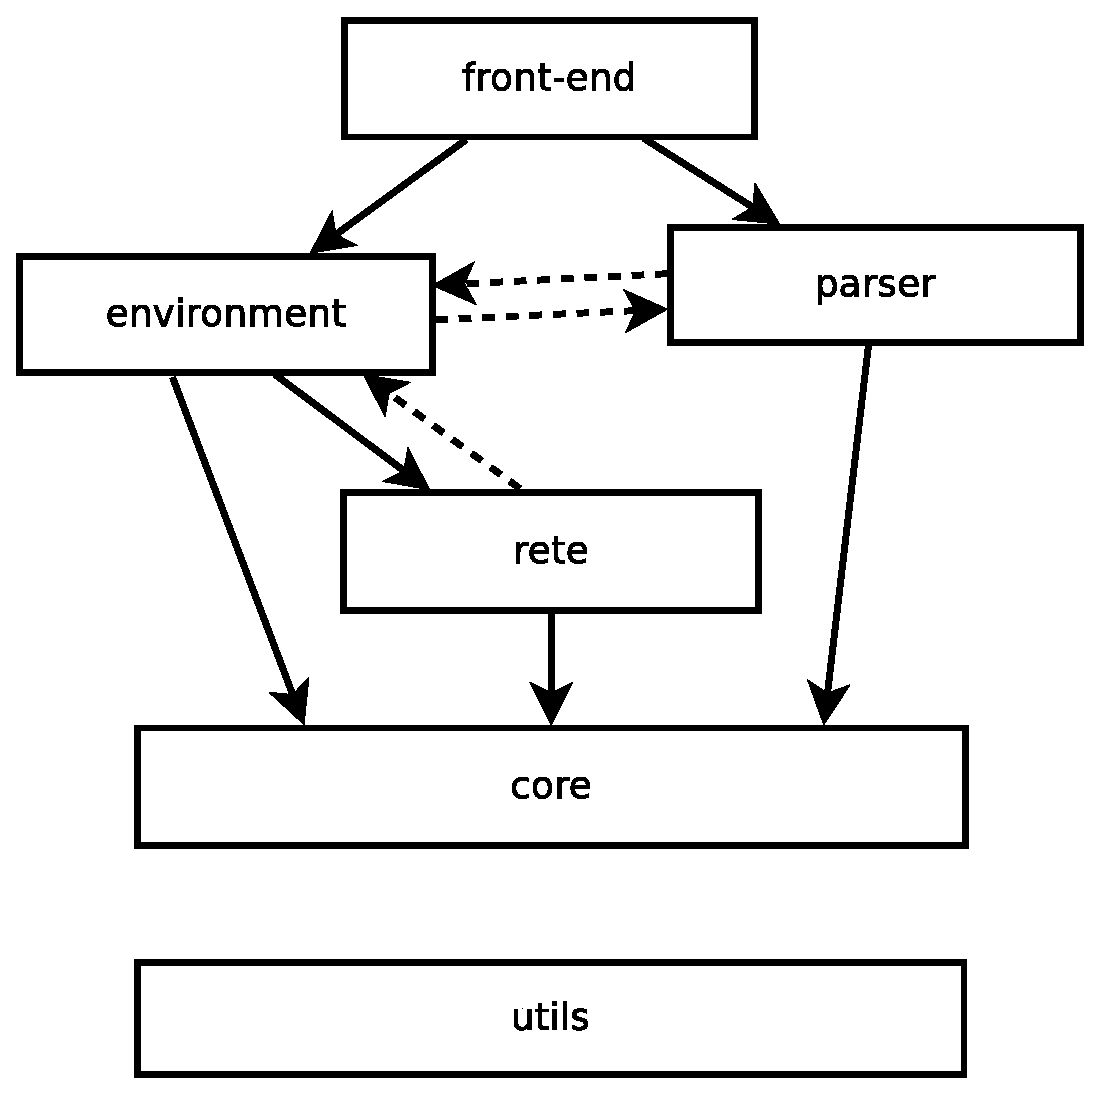
\includegraphics[height=10cm]{modules.eps}
\caption{Architektura ExiLu}
\label{modules}
\end{figure}

Obrázek \ref{modules} zobrazuje architekturu knihovny ExiL, tedy moduly, do
kterých je kód knihovny rozdělen, a jejich vzájemnou komunikaci. Orientace šipek
určuje směr volání funkcí (metod, maker) poskytovaných moduly, např. modul
\verb|front-end| volá funkce modulu \verb|parser| a ne naopak. Těmito voláními
jsou zároveň definovány závislosti mezi moduly, ty mají tedy stejnou orientaci.

Modul \verb|utils| definuje různorodé pomocné funkce a makra, která jsou volána
všemi ostatními moduly. V obrázku \ref{modules} bych tedy mohl zahrnout šipky ze
všech ostatních modulů do modulu \verb|utils|, to by jej však činilo zbytečně
nepřehledným. Většina funkcí a maker, která modul definuje, usnadňuje
nízkoúrovňovou práci se symboly a datovými strukturami - (asociativními)
seznamy, množinami, stromy, \emph{hashovacími tabulkami} apod.

Modul \verb|core| definuje základní objekty, s nimiž zbytek knihovny
pracuje. Ty reprezentují fakty, vzory, šablony a pravidla. Fakty a vzory jsou
definovány ve dvou variantách - jednoduché a strukturované, jak jsem uvedl v
uživatelské příručce.

Modul \verb|rete| implementuje algoritmus RETE, který slouží k efektivnímu
vyhodnocování podmínek odvozovacích pravidel. Algoritmus je implementován
\emph{dataflow} sítí, jejíž fungování popíšu detailně v kapitole \ref{rete}
Algoritmus RETE je sice nejkomplexnější částí ExiLu, veřejné rozhraní modulu
\verb|rete| je však velmi jednoduché.

Modul poskytuje dvojici metod, kterými síť RETE upozorníme na přidání nebo
odebrání pravidel. Ty dle potřeby doplní síť o uzly potřebné k vyhodnocení
podmínek těchto pravidel, případně uzly při odebrání pravidla odstraní.

Další dvojice metod upozorní síť na přidání faktu do (resp. odebrání z) pracovní
paměti. Síť pak přepočítá splněné podmínky pravidel a případně upozorní
prostředí na nově přibyvší nebo rozbité shody (\emph{broken match} - pravidla,
která byla splněná nějakou posloupností faktů a už nejsou).

Modul \verb|environment| definuje stejnojmenný objekt, který udržuje průbežný
stav prostředí a řídí průběh inference. Hodnoty, které stav prostředí tvoří,
jsem popsal v kapitole \ref{env cleanup} Prostředí udržuje krom jiného
referenci na síť \verb|rete|, kterou upozorňuje na nastalé změny.

Modul \verb|parser| zajišťuje vytváření \verb|core| objektů z externí
reprezentace (té, kterou předáváme funkcím a makrům při práci s knihovnou).
Modul rozpoznává jak základní, tak CLIPSovou syntax, takže o to, kterou z nich
uživatel používá, se zbytek kódu nemusí dále starat.

Při parsování strukturovaných faktů či vzorů se \verb|parser| dotazuje
aktuálního prostředí na definici šablony. Při zpětné inferenci prostředí
vyhodnocuje volání \verb|assert| v důsledcích pravidel a žádá \verb|parser| o
zparsování reprezentací faktů v~nich. Proto jsem mezi moduly \verb|environment|
a \verb|parser| přidal šrafované šipky. Kromě těchto nutných interakcí spolu
však moduly nekomunikují.

Modul \verb|front-end| udržuje seznam definovaných prostředí a ví, které je
právě aktivní. Kromě manipulace tohoto seznamu modul sám žádnou funkcionalitu
neimplementuje. Pouze kvotuje parametry předané makrům, předává je
\verb|parser|u a~výsledné objekty (se zbytkem parametrů) pak aktivnímu prostředí.

Do diagramu jsem nezahrnul modul \verb|gui|. Ten implementuje grafické
uživatelské rozhraní a poskytuje dvě metody - \verb|show-gui| a
\verb|update-lists|. Rozhraní se dotazuje prostředí, se kterým je svázáno, na
hodnoty aktuálního stavu a je jím upozorněno, pokud se tyto změní.

\subsubsection{Algoritmus RETE}
\label{rete}

Algoritmus RETE slouží k efektivnímu vyhodnocování splnění podmínek odvozovacích
pravidel (dále jen vyhodnocování). Je implementován dataflow sítí. Ta je
rozdělena do dvou částí, označovaných jako alpha a beta. Alpha část sítě
vyhodnocuje splnění jednotlivých podmínek pravidla fakty nově přidanými do či
odebranými z pracovní paměti. Beta část pak zajišťuje zachování konzistence
vazeb proměnných mezi podmínkami.

To, že je vyhodnocování sítí RETE tak efektivní, je zajištěno maximálním
sdílením častí sítě mezi pravidly. Mají-li dvě pravidla strukturálně stejný vzor
nějaké podmínky (liší se jen použité proměnné), sdílí tato pravidla část alpha
sítě, která tuto podmínku vyhodnocuje. Pokud mají dvě pravidla stejných několik
prvních podmínek, sdílí tato pravidla kromě části alpha sítě i část beta sítě,
která zajišťuje konzistenci vazeb proměnných mezi nimi.

Dataflow síť je tvořena uzly. Jejich vzájemné interakce nazýváme
v~algoritmu aktivacemi. Každý uzel má několik sousedů. Aktivace však v síti
probíhají jen jedním směrem. Uzly, které jsou daným uzlem aktivovány, budu
nazývat jeho potomky. Uzly rozdělujeme na dva základní typy - paměťové a
testovací. Paměťové uzly ukládají průběžné výsledky vyhodnocování. Testovací
uzly provádějí různé typy testů (v závislosti na typu uzlu), nutných pro
vyhodnocení podmínek pravidla.  Uzlu je při aktivaci vždy předána nějaká datová
struktura. Tou je buď fakt, nebo token, který reprezentuje posloupnost faktů.
Zatímco paměťové uzly po aktivaci a uložení datové struktury do své paměti vždy
aktivují své potomky, testovací uzly aktivují potomky jen v případě úspěšného
testu.

\begin{figure}[h]
\centering
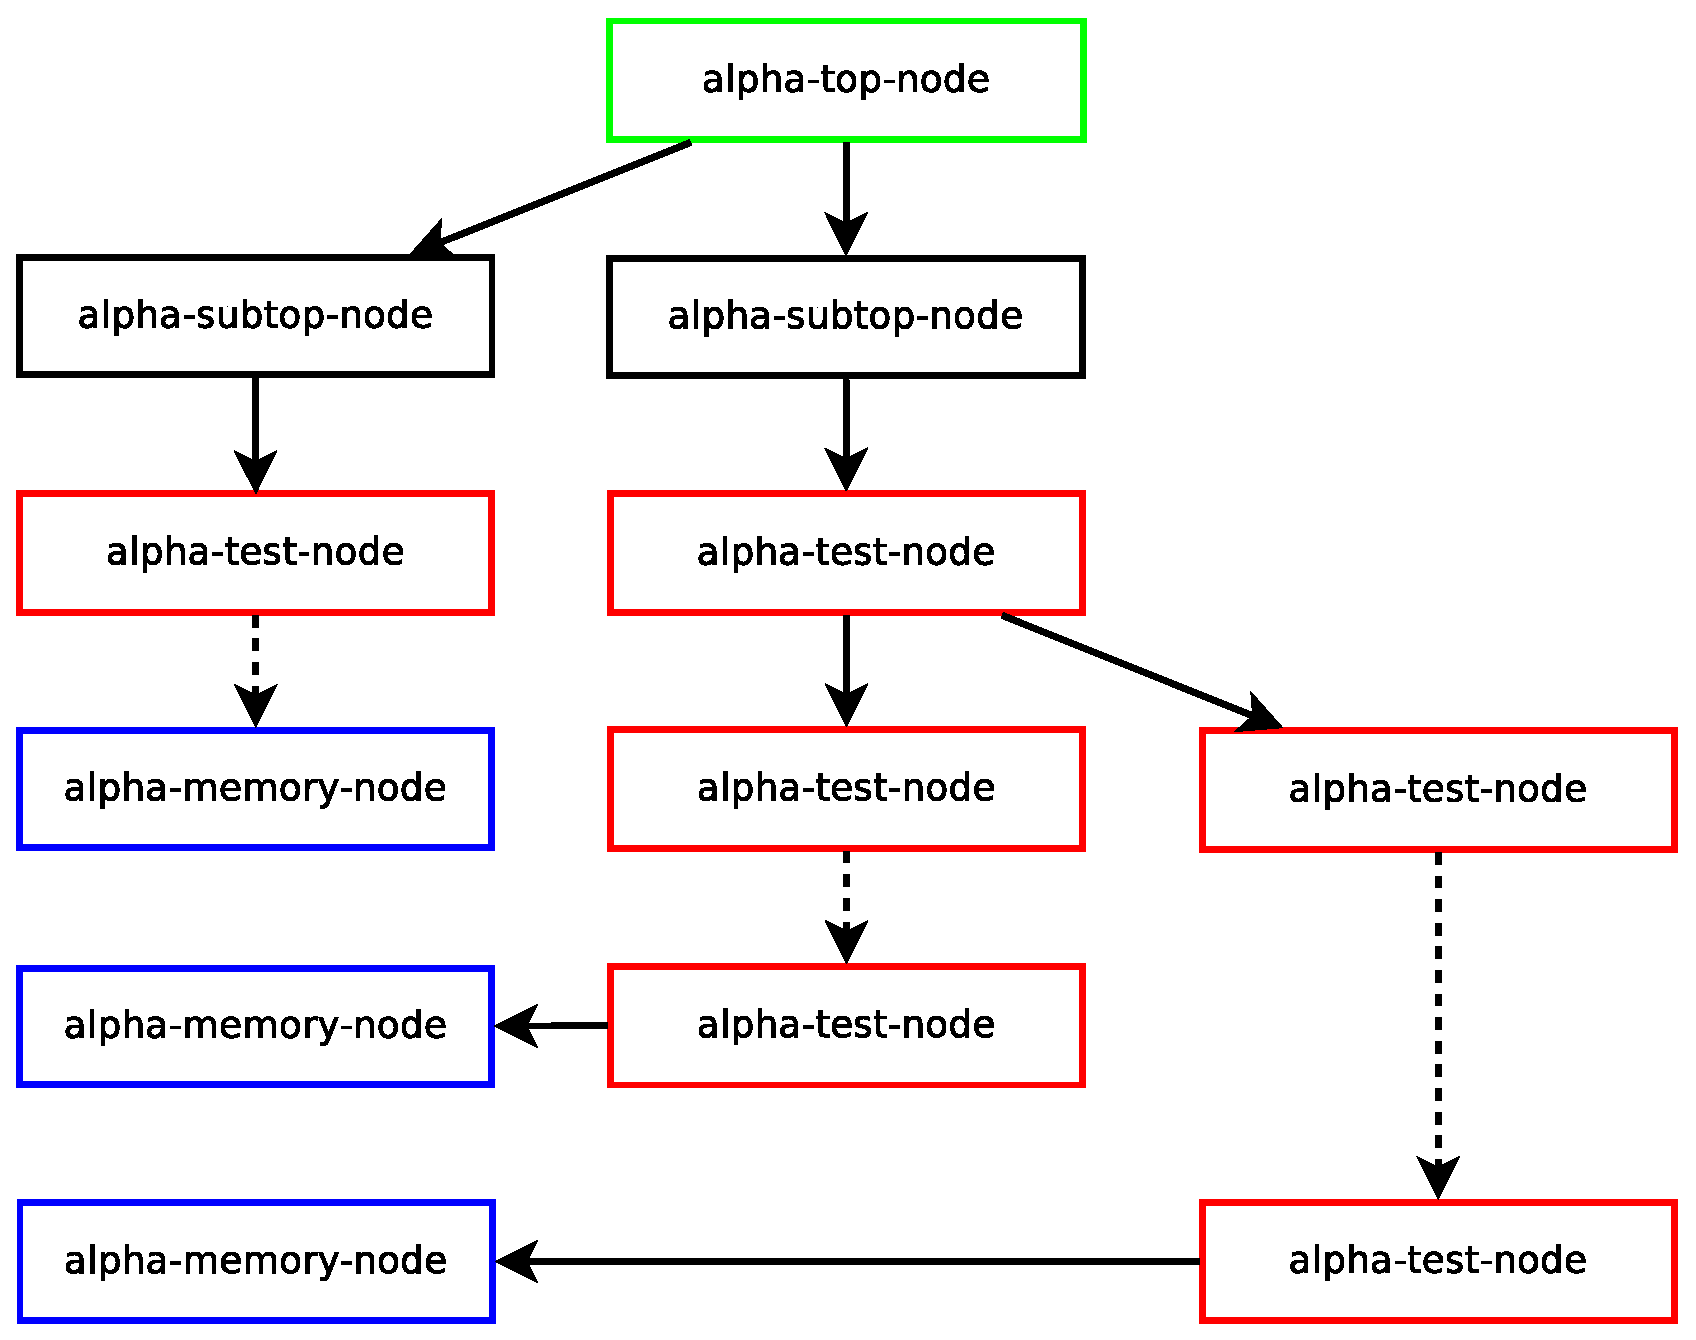
\includegraphics[height=10cm]{rete-alpha.eps}
\caption{Alpha část sítě RETE}
\label{rete-alpha}
\end{figure}

Obrázek \ref{rete-alpha} zobrazuje úsek alpha části sítě RETE. Uzel
\verb|alpha-top-node| je vstupním bodem této sítě. Ten je aktivován při každé
změně pracovní paměti faktem, který byl přidán nebo odebrán. Potomky
\verb|alpha-top-nodu| jsou \verb|alpha-subtop-nody|, jeden pro jednoduché fakty
a jeden pro každou definovanou šablonu. \verb|alpha-top-node| aktivuje příslušný
\verb|alpha-subtop-node| podle typu faktu.

Každá cesta z \verb|alpha-subtop-nodu| do \verb|alpha-memory-nodu| skrze
posloupnost \verb|alpha-test-nodů| vyhodnocuje jednu podmínku nějakého pravidla
(případně skupiny pravidel). Mějme např. pravidla
\begin{minted}{cl}
(defrule rule1
  (in :object box :location ?locaction)
  =>
  ...)
(defrule rule2
  (in :object box :location ?loc)
  =>
  ...).
\end{minted}
Tato pravidla mohou sdílet část alpha sítě pro vyhodnocení svých podmínek, neboť
ty se liší pouze názvy proměnných. Pro vyhodnocení těchto podmínek budeme
potřebovat jeden \verb|alpha-subtop-node| pro šablonu \verb|in|, jeden
\verb|alpha-test-node| pro testování, zda je hodnota slotu \verb|object| rovna
hodnotě \verb|box| a jeden \verb|alpha-memory-node| pro uložení faktů, které
tuto podmínku splňují. Pro slot \verb|location| \verb|alpha-test-node|
nepotřebujeme, neboť alpha část sítě se hodnotami proměnných nezabývá.

\begin{figure}[h]
\centering
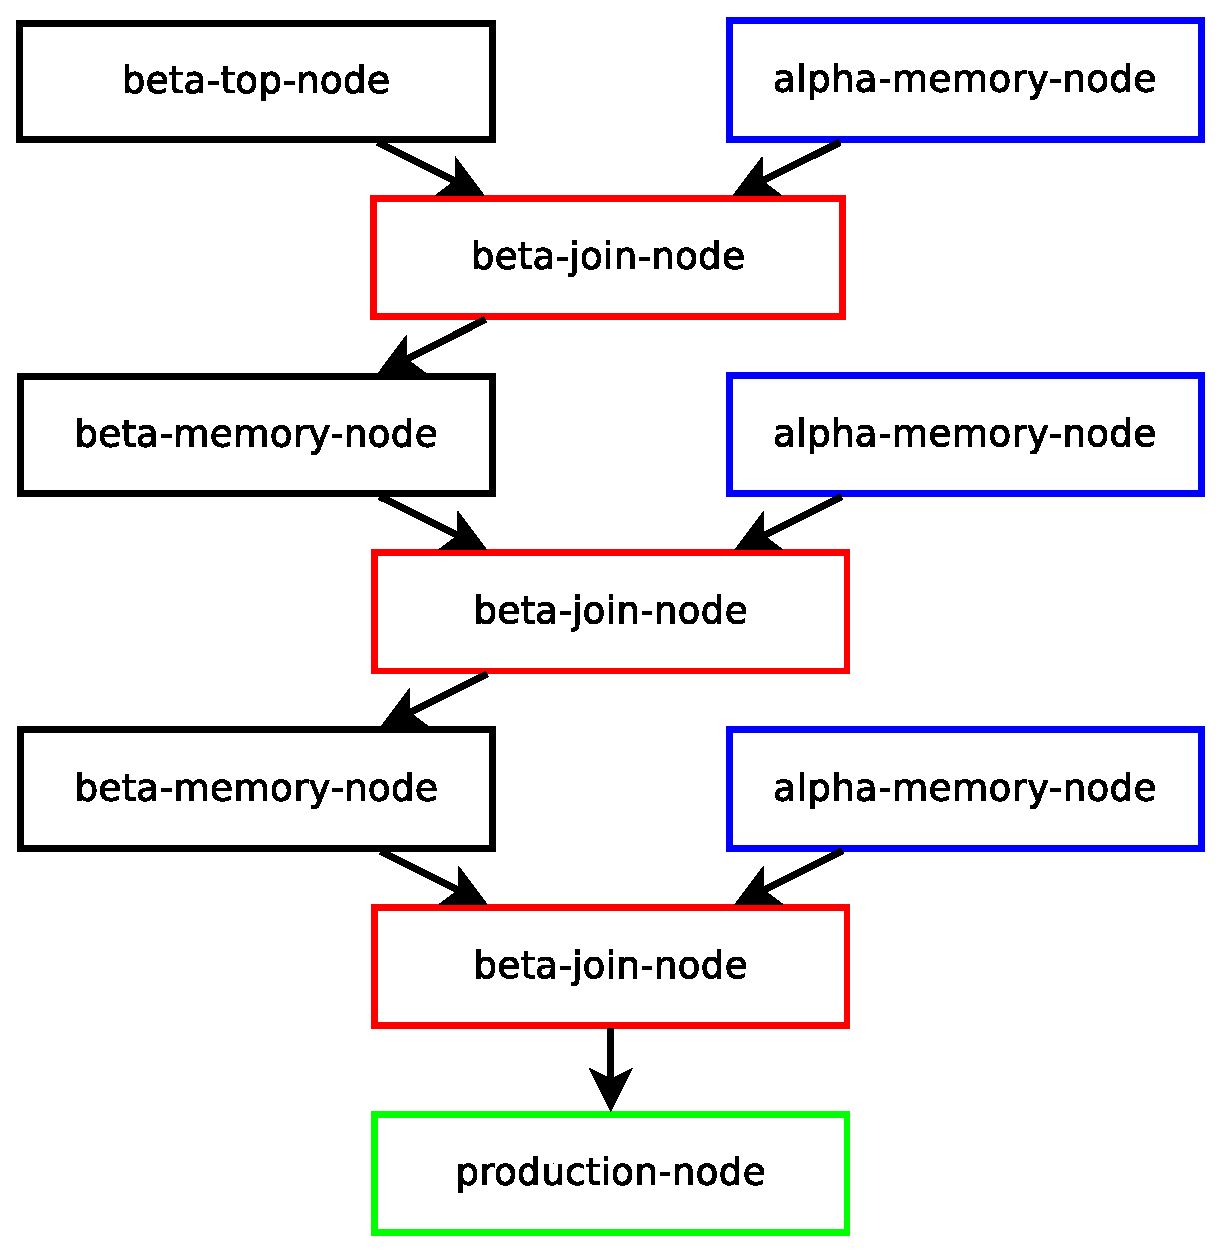
\includegraphics[height=10cm]{rete-beta.eps}
\caption{Beta část sítě RETE}
\label{rete-beta}
\end{figure}

Obrázek \ref{rete-beta} zobrazuje úsek beta části sítě, spolu s
\verb|alpha-memory-nody|, kterými sem vstupují fakta splňující jednotlivé
podmínky pravidel. Každý \verb|beta-memory-node| udržuje množinu tokenů
reprezentujících posloupnosti faktů, z nichž každý splňuje podmínku nějakého
pravidla. \verb|beta-join-nody| pak testují konzistenci vazeb proměnných mezi
těmito podmínkami. \verb|beta-top-node| je speciální případ
\verb|beta-memory-nodu|, který udržuje v paměti pouze jeden prázdný token.
\verb|production-node| je pak speciální případ \verb|beta-memory-nodu|, který
při aktivaci upozorní prostředí, že byly splněny všechny podmínky pravidla,
případně že po odstranění faktu už nejsou všechny splněny.

Mějme například pravidlo
\begin{minted}[samepage]{cl}
(defrule rule
  (goal :object ?obj :from ?from :to ?to)
  (in :object ?obj :location ?from)
  (in :object robot :location ?to)
  =>
  ...).
\end{minted}
Alpha část sítě pro toto pravidlo bude obsahovat tři \verb|alpha-memory-nody|,
každý pro jednu jeho podmínku (kdyby však byla v poslední podmínce místo hodnoty
\verb|robot| proměnná, vystačili bychom si se dvěma \verb|alpha-memory-nody|).

Beta část sítě bude vypadat tak, jako na obrázku \ref{rete-beta}
První (shora) \verb|beta-test-node| ve skutečnosti nemá co testovat, neboť jde o
první podmínku pravidla. První \verb|beta-memory-node| bude udržovat tokeny
délky 1 reprezentující \uv{posloupnost} faktů, které splňují první podmínku.
Druhý \verb|beta-join-node| bude testovat konzistenci vazeb mezi druhou
a první podmínkou pravidla. Druhý \verb|beta-memory-node| bude udržovat tokeny
délky 2 reprezentující dvojice faktů, splňující první dvě podmínky pravidla.
Třetí \verb|beta-join-node| bude testovat konzistenci vazeb mezi třetí podmínkou
pravidla a předchozími dvěma. \verb|production-node| pak bude udržovat tokeny
délky 3 reprezentující trojice faktů splňující všechny podmínky pravidla.

% Druhý \verb|beta-test-node| je aktivován buď zleva \verb|alpha-memory-nodem|,
% přibyde-li fakt, který splňuje druhou podmínku pravidla, nebo zprava
% \verb|beta-memory-nodem|, přibyde-li fakt, který splňuje první podmínku.

Přidávejme nyní postupně fakty do pracovní paměti. Přidáním
\verb|(in :object box :location A)| dojde (po průchodu alpha částí sítě) k
aktivaci druhého \verb|alpha-memory-nodu|. Ten uloží fakt do své paměti
a aktivuje \uv{zprava} druhý \verb|beta-join-node|. Ten prohledá paměť
\verb|beta-memory-nodu| nad sebou, zda neobsahuje nějaký token s
konzistentními vazbami proměnných. Ta je ale prázdná, takže zde se aktivace
zastaví.

Přidáním \verb|(goal :object box :from A :to B)| dojde k aktivaci prvního
\verb|alpha-memory-nodu|. Ten po uložení faktu aktivuje první
\verb|beta-join-node|. Ten nemá co testovat, takže aktivuje
\verb|beta-memory-node| pod sebou. Ten uloží jednoprvkový token s přidaným
faktem a aktivuje opět druhý \verb|beta-join-node|, tentokrát však \uv{zleva}.
\verb|beta-join-node| tentokrát prohledá obsah paměti \verb|alpha-memory-nodu|
nad sebou, zda neobsahuje fakt konzistentní s tokenem. \verb|beta-join-node| zde
testuje, zda jsou hodnoty slotů \verb|object| a \verb|location| faktu v alpha
paměti shodné s hodnotami \verb|object| a \verb|from| prvního faktu tokenu v
beta paměti.

Test zde skončí úspěšně, takže druhý \verb|beta-join-node| aktivuje
\verb|beta-memory-node| pod sebou a předá mu dvouprvkový token s oběma fakty.
Ten aktivuje třetí \verb|beta-join-node| \uv{zleva}. Ten následně prohledá paměť
\verb|alpha-memory-nodu| nad sebou. Ta je ale prázdná, takže zde aktivace skončí.

Po přidání faktu \verb|(in :object robot :location B)| dojde k aktivaci třetího
\verb|alpha-memory-nodu|. Ten fakt uloží a aktivuje třetí \verb|beta-join-node|
\uv{zprava}. Ten prohledá paměť \verb|beta-memory-nodu| nad sebou, zda
neobsahuje konzistentní tokeny. Ta obsahuje dvouprvkový token s prvními dvěma
fakty. \verb|beta-join-node| tedy srovná hodnotu slotu \verb|location| přidaného
faktu s hodnotou \verb|to| prvního faktu tokenu. Protože tyto hodnoty se
shodují, aktivuje \verb|beta-join-node| \verb|production-node| pod sebou a předá
mu tříprvkový token s posloupností faktů, které splňují všechny podmínky
pravidla. Ten token uloží a upozorní prostředí, že pravidlo bylo splňeno
posloupností faktů v tokenu.

\subsubsection{Kompozitní podmínky pravidel}

Podporu kompozitních podmínek odvozovacích pravidel (vnořené aplikace logických
funkcí v podmínkách) jsem v ExiLu neimplementoval. Rád bych zde ale ukázal, proč
je implementace této funkcionality vzhledem k aktuální implementaci algoritmu
RETE složitá.

\begin{figure}[h]
\centering
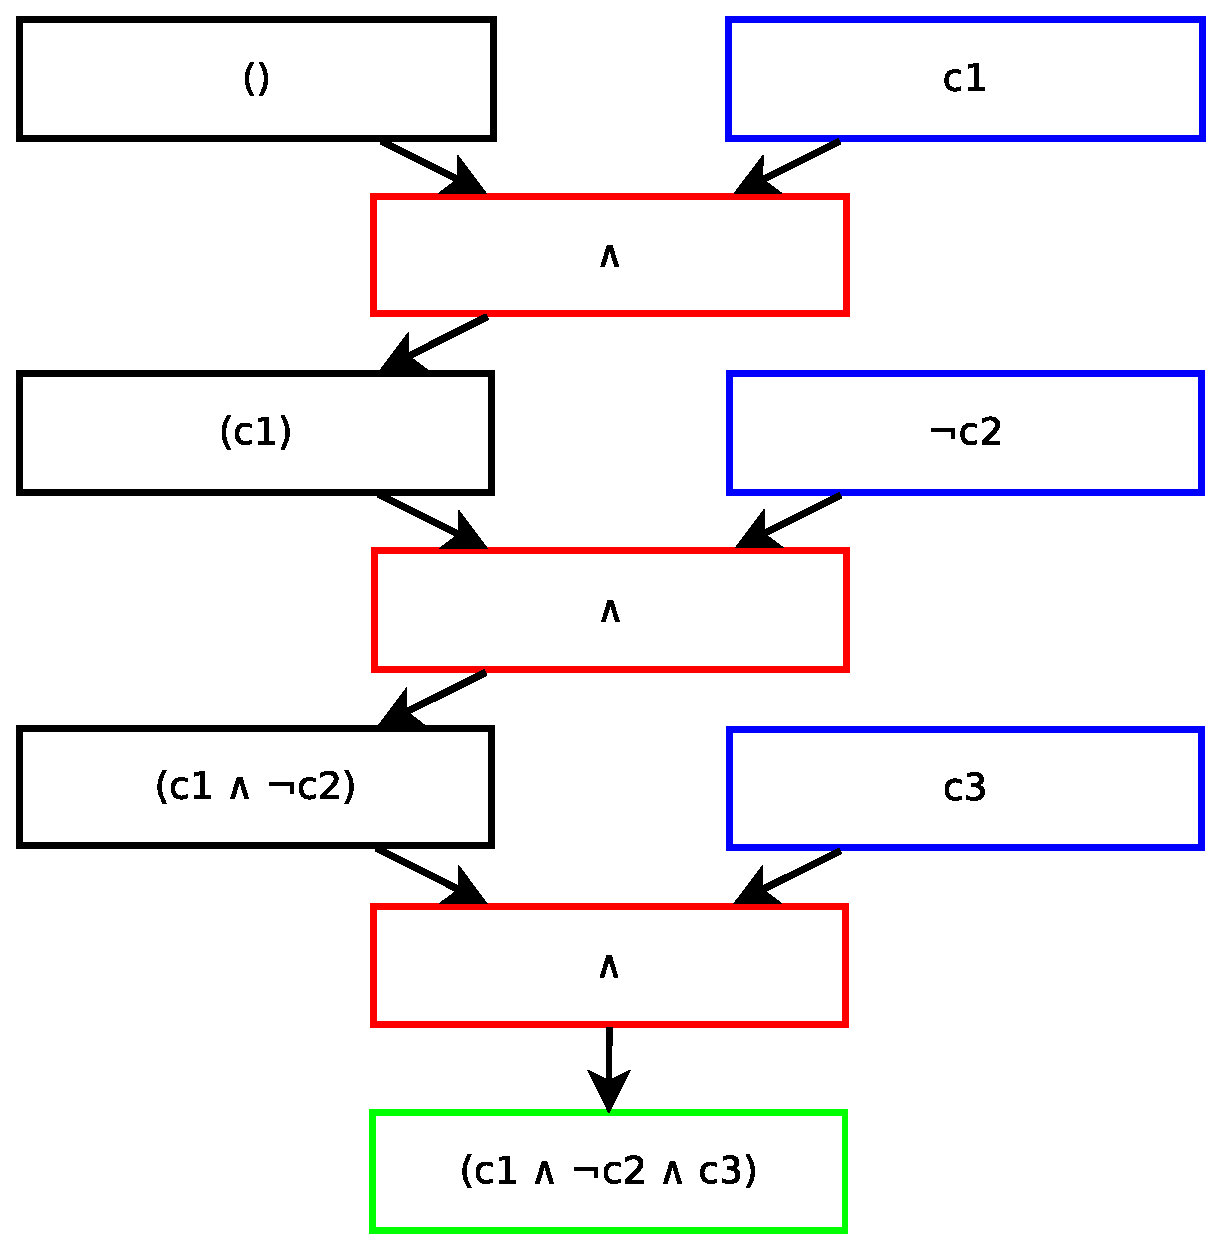
\includegraphics[height=10cm]{rete-beta-conds.eps}
\caption{Beta část sítě RETE s funkcemi uzlů}
\label{rete-beta-conds}
\end{figure}

Obrázek \ref{rete-beta-conds} ukazuje diagram beta části sítě RETE z předchozí
sekce. Názvy uzlů jsem zde ale nahradil jejich funkcí. Paměťové uzly ukládají
fakty nebo tokeny splňující jednu (v případě alpha-memory-nodů), nebo více (u
beta-memory-nodů) podmínek pravidla. Testovací (beta-join-nody) pak zajišťují
agregaci těchto faktů a tokenů. Jednu z podmínek jsem navíc pro ukázku znegoval.

Síť v diagramu splňuje několik podmínek:
\begin{enumerate}
  \item uzly jsou konstruovány ve stejném pořadí, v jakém se podmínky v definici
    pravidla vyskytují,
  \item beta-join-node vždy spojuje jeden alpha-memory-node s jedním
    beta-memory-nodem, agreguje tedy fakty splňující jednu podmínku pravidla s
    tokeny reprezentujícími posloupnost faktů splňující jeho předchozí podmínky,
  \item negace podmínky je vždy aplikována jen na úrovni jednoho faktu.
\end{enumerate}

\begin{figure}[h]
\centering
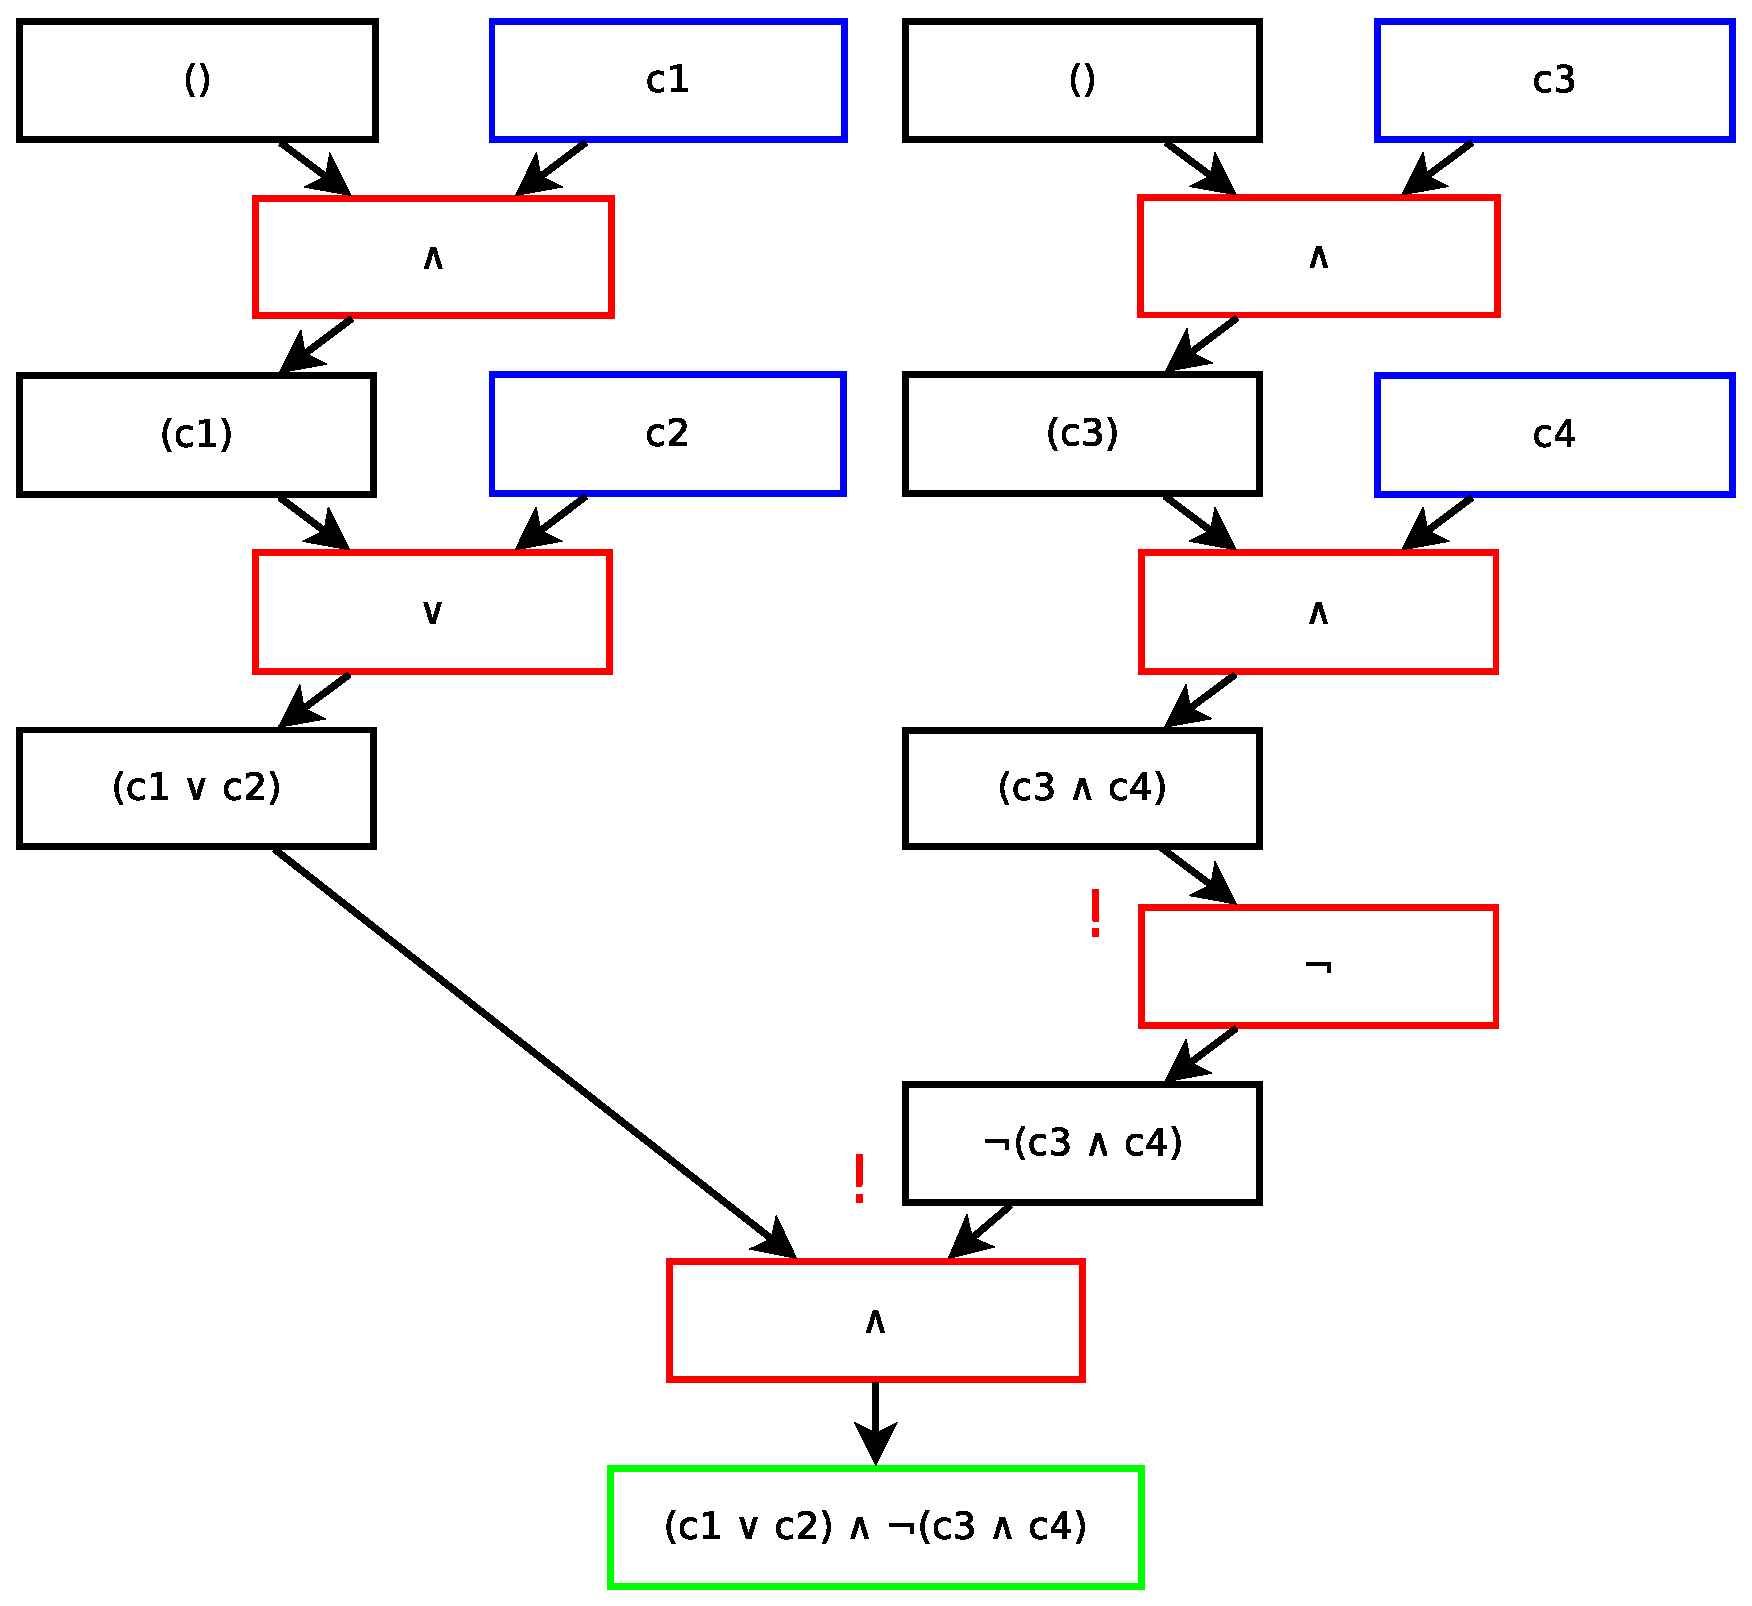
\includegraphics[height=12cm]{rete-beta-comp-conds.eps}
\caption{Síť RETE s kompozitními podmínkami}
\label{rete-beta-comp-conds}
\end{figure}

Představme si nyní stavbu RETE sítě v případě následujícícho pravidla
s~kompozitními podmínkami:
\begin{minted}{cl}
(defrule rule
  (and (or condition1 condition2)
       (not (and condition3 condition4)))
  =>
  ...)
\end{minted}
Ta je zobrazena na obrázku \ref{rete-beta-comp-conds} Z diagramu vidíme, že síť porušuje všechny
uvedené podmínky.

\begin{framed}
  \begin{itemize}
    \item popsat, co je problematického na podpoře této sítě
    \item podmínky třeba procházet rekurzivně a síť budovat stromovitě
    \item token je nyní list, stačí to, nebo musí být také strom?
    \item testy v join nodech nyní ukládají pozici - o kolik podmínek zpět,
      který atom v přechozí, který atom v aktuální
    \item pozice by musela mít u beta-beta joinu minimálně jednu pozici navíc -
      (fakt,atom)-(fakt,atom), pokud by musel být token strom, ještě složitější
    \item lze vyřešit join-nody obecně - beta-beta i beta-alpha, nebo nutné dva
      typy?
    \item jak reprezentovat node, který neguje složenou podmínku?
    \item jak joinovat tokeny, které mohou zahrnovat výsledky negativní podmínky?
    \item síť je cyklická a jako taková špatně vizualizuje
    \item počet uzlů sítě roste velmi rychle $\rightarrow$ mnoho uzlů i při
      několika pravidlech $\rightarrow$ náročné ladění
    \item podpora kompozitních podmínek je navíc problematická vzhledem ke
      zpětné inferenci (ale ta už je stejně omezená) - znamenalo by složené cíle
      (kvůli or, not)
    \item zmínit, jak jednoduchá je implementace, pokud podmínky pracují pouze
      se substitucemi proměnných - bez rete
  \end{itemize}
\end{framed}
% Z fungování beta částí sítě RETE (viz sekce \ref{rete}) vidíme, že vyhodnocování
% podmínek pravidla je inherentně sekvenční. \verb|Beta-join-nody| zde
% implementují logickou spojku \emph{a} mezi podmínkami pravidla, která je zde
% zleva asociativní.

\subsubsection{Undo/redo}
Možnost vrácení provedených akcí a jejich opětovného provedení (undo/redo) je
implementována na úrovni prostředí, které udržuje aktuální stav systému.
Hodnoty, které stav tvoří, jsem popsal v sekci \ref{env cleanup} a možnosti,
které undo/redo poskytuje, v sekci \ref{undo}

Prostředí je v programu reprezentováno objektem \verb|environment|. Stav
prostředí je uchováván ve slotech tohoto objektu.

Prostředí dále udržuje dva zásobníky - \verb|undo| a \verb|redo|.
Každý z~těchto zásobníků ukládá seznamy tvořené popiskem akce k vrácení,
uzávěrem, který akci vrátí a~uzávěrem, který ji opět provede. První uzávěr ve
svém lexikálním prostředí uchovává hodnoty potřebné k vrácení akce. Zásobníky
jsou manipulovány pouze několika makry a metodami k tomu určenými, zbytek kódu k
zásobníkům přímo nepřistupuje.

Tělo každé akce, která mění hodnoty prostředí, je obaleno buď voláním makra
\verb|with-undo|, nebo \verb|with-saved-slots|. Volání \verb|with-undo| je kromě
těla akce předán uzávěr, který zajistí její vrácení. Makro \verb|with-undo|
po vyhodnocení těla akce zajistí, že se na zásobník \verb|undo| uloží předaný
uzávěr spolu s uzávěrem, který akci opět provede při volání \verb|redo|.
Tento druhý uzávěr pouze vyhodnotí původní tělo akce.

Makro \verb|with-saved-slot| zjednodušuje volání \verb|with-undo|. Toto makro
bere kromě těla akce seznam slotů prostředí, které je třeba před akcí uložit.
Makro pak automaticky vytvoří uzávěr, který předá makru \verb|with-undo|. Tento
uzávěr si ve svém lexikálním prostředí pamatuje kopie původních hodnot požadovaných
slotů prostředí a při vyhodnocení je nastaví zpět na tyto hodnoty.

Prostředí ke každému svému slotu definuje metodu \verb|copy-<slot>|, např.
\verb|copy-facts|. Makro \verb|with-saved-slots| tedy vytvoří potřebný uzávěr
tak, že v \verb|let|u naváže výsledky volání těchto metod pro každý požadovaný
slot. V tomto \verb|let|u pak vytvoří anonymní (lambda) funkci, která hodnoty
prostředí nastaví zpět na ty, které \verb|let| navázal.

Funkce \verb|undo| pak jednoduše odstraní seznam z vrcholu zásobníku
\verb|undo|, zavolá uzávěr, který vrátí poslední akci a druhý uzávěr, který akci
opět provede, uloží na vrchol zásobníku \verb|redo|. Funkce \verb|redo| funguje
symetricky.

Nakonec je třeba zajistit, aby každé volání \verb|with-undo| uložilo na zásobník
právě jeden uzávěr k vrácení akce. Například pokud samostatně voláme makro
\verb|assert| pro přidání nějakého faktu do pracovní paměti, chceme, aby toto volání
bylo možné vrátit. Pokud ale voláme \verb|step|, jehož výsledkem je aktivace
nějakého pravidla, které ve svých důsledcích volá makro \verb|assert|, chceme,
aby se volání \verb|step| uložilo na zásobník jako jedna akce. Volání
\verb|assert|, ke kterému v průběhu této akce dojde, už samostatně ukládat
nechceme.

K tomuto účelu definuje prostředí dynamickou proměnnou \verb|*undo-enabled*|.
Makro \verb|with-undo| ukládá uzávěr na zásobník jen v případě, že je hodnota
této proměnná \verb|true|. Tělo akce pak makro vyhodnocuje s hodnotou této
proměnné navázanou na \verb|false|. Tím je zajištěno, že se uzávěr na zásobník
\verb|undo| uloží vždy jen v \uv{nejvnějšnějším} volání makra \verb|with-undo|.

Díky makrům \verb|with-undo| a \verb|with-saved-slots| je možné velmi snadno
přidat do prostředí další akce s možností jejich vrácení. Stačí jen tělo akce
obalit jedním z těchto maker bez nutnosti vědět, jak je vrácení akce
implementováno. Pokud potřebujeme do prostředí přidat další slot, jehož hodnotu
je třeba při volání \verb|undo| obnovovat, stačí k tomuto slotu implementovat
metodu \verb|copy|.

Nejsložitějším problémem při implementaci vracení akcí bylo implementovat metodu
\verb|copy-rete|. Ta kopíruje dataflow síť RETE uloženou ve slotu \verb|rete|
prostředí. Kopírovnání sítě RETE je složité, neboť síť obsahuje cykly. Síť se
sice z~pohledu aktivace uzlů chová jako acyklický graf, některé uzly však
uchovávájí reference na své sousedy proti směru hran tohoto grafu.

Pro účely kopírování sítě RETE jsem implementoval obecnou metodu vyššího řádu
pro průchod cyklickým grafem. Tato metoda využívá techniky
memoizace\footnote{\url{http://en.wikipedia.org/wiki/Memoization}}. Metoda bere
kromě výchozího uzlu grafu tři funkce, které aplikuje na navštěvované uzly před
memoizací a jimiž zajišťuje agregaci hodnot vrácených sousedy uzlu.

Fungování metody je pro textový popis příliš složité, považuji ji však za jednu
z nejzajímavějších částí nového kódu, hlavně díky její obecnosti. Zrojový kód
metody je v souboru \verb|rete/graph-traversal.lisp|, kód kopírující síť rete,
který metodu využívá pak v souboru \verb|rete/rete-copy.lisp|. Celkově je kód
zajišťující kopírování sítě RETE asi třikrát delší, než zbytek kódu
implementující funkcionalitu undo/redo.

\subsubsection{Zpětná inference}

Zpětná inference hledá odpovědi na základě zadaných cílů. Odpovědi jsou zde
reprezentovány použitou substitucí proměnných v cílech a posloupností faktů
a~pravidel, použitých k jejich splnění. Možnosti zpětného řetězení a způsob jeho
použití jsem popsal v sekci \ref{backward inference}

Kód implementující zpětnou inferenci pracuje se dvěma datovými strukturami -
seznamem cílů a zásobníkem pro backtracking (návrat ve výpočtu, pokud daná cesta
nevede ke splnění všech cílů, nebo pro hledání alternativních odpovědí). Program
nemodifikuje pracovní paměť, ani nevyhodnocuje odvozovací pravidla, pouze
analyzuje volání \verb|assert| v jejich důsledcích.

Cíle jsou v programu reprezentovány vzory, podobně jako podmínky pravidel.
Inferenci si tedy můžeme představit tak, jako bychom definovali jedno pravidlo,
jehož podmínky reprezentují seznam cílů a hledali všechny možné cesty výpočtu,
vedoucí k jeho splnění.

Zásobník pro backtracking (dále jen zásobník) ukládá struktury, z nichž každá
reprezentuje právě provedený krok výpočtu. Tato struktura je tvořen aktuálním
seznamem cílů, faktem či pravidlem, použitým pro splnění aktuálního cíle a
seznamem faktů a pravidel, která již byla pro splnění tohoto cíle použita (v
případě návratu výpočtu).

Zpětná inference je řízena třemi metodami prostředí - \verb|back-step|,
\verb|backtrack| a \verb|back-run|. Metoda \verb|back-step| vybere první cíl ze
seznamu a hledá nejprve fakta, poté pravidla, vedoucí k jeho splnění, přičemž
ignoruje ta, která už byla pro splnění cíle dříve použita.

Při hledání faktů, která splňují cíl, srovnáváme fakt se vzorem cíle podobně,
jako při vyhodnocování podmínek pravidel při dopředné inferenci (viz sekce
\ref{inference}). Výsledkem tohoto srovnání je v případě shody substituce
proměnných, vyskytujících se ve vzoru cíle. Je-li nalezen fakt, který aktuální
cíl splňuje, program uloží nalezenou shodu na zásobník, načež cíl odstraní ze
seznamu cílů a~aplikuje použitou substituci proměnných na zbytek cílů. Není-li
nalezen takový fakt, uvažuje program dále odvozovací pravidla.

Při hledání pravidel, která vedou ke splnění aktuálního cíle, program zohledňuje
všechna volání \verb|assert| v jejich důsledcích. Reprezentace faktů, použité ve
voláních \verb|assert|, nechá program zpracovat \verb|parser|em a výsledné fakty
pak srovnává se vzorem cíle podobně, jako fakty v pracovní paměti. Protože jde
však o~důsledkovou část pravidla, volání \verb|assert| mohou obsahovat proměnné.
Program tedy hledá unifikaci aktuálního cíle s tímto \uv{proměnným faktem}.

V případě shody je výsledkem unifikace opět substituce proměnných. Program v
tomto případě opět uloží shodu na zásobník, odstraní aktuální cíl ze seznamu a
aplikuje použitou substituci proměnných na zbytek cílů. Nejpreve ale program
přidá podmínky použitého pravidla do seznamu cílů. Podmínky použitého pravidla
se tedy stávají dalšími cíli, které je třeba splnit, abychom nalezli hledanou
odpověď.

Hledání unifikace vzoru cíle s \uv{proměnným faktem} je podobné jako v jazyce
Prolog. Je však jednodušší o to, že symbolická reprezentace faktů a vzorů je
lineární (seznamy nejsou vnořené) a není třeba rozlišovat mezi relačními
a~funkčními symboly. V případě strukturovanch faktů a vzorů jsou jednotlivé
sloty srovnávány, jako by šlo o atomy seznamu, jen zde nezáleží na pořadí, nýbrž
se srovnávají odpovídající sloty faktu a vzoru.

Pokud metoda \verb|back-step| nenalezne fakt ani pravidlo vedoucí ke splnění
aktuálního cíle, volá metodu \verb|backtrack|. Ta odstraňuje postupně struktury z
vrcholu zásobníku, obnoví cíle do stavu při uložení struktury a hledá shody s
dosud nepoužitými fakty a pravidly. Pokud takovou shodu nalezne, ubírá se
výpočet dále touto cestou. Je-li celý zásobník vyčerpán před nalezením shody,
nahlásí metoda neúspěch.

Metoda \verb|back-run| volá opakovaně metodu \verb|back-step|, dokud nejsou
splněny všechny cíle, nebo není nahlášen neúspěch. V případě, že už jsou všechny
cíle splněny, volá \verb|back-step| metodu \verb|backtrack| pro nalezení
alternativních odpovědí. To může vést k nalezení nové shody, nebo vyčerpání
zásobníku, což znamená, že už žádné další odpovědi neexistují.

Dospěje-li volání \verb|back-run| ke splnění všech cílů, vytiskne se seznam
faktů a~pravidel, použitých ke splnění jednotlivých cílů. Dále se vytiskne
substituce proměnných, která byla pro splnění cílů použita. Tato substituce je
tvořena složením všech substitucí, použitých v jednotlivých krocích výpočtu. Ve
výsledné substituci jsou ponechány pouze proměnné, které uživatel použil v
definicích původních cílů. Průběžné proměnné, které se sem dostaly při aplikaci
odvozovacích pravidel nejsou pro uživatele zajímavé.

Implementace zpětné inference je inspirována prohledáváním SLD-stromů používaným
v jazyce
Prolog\footnote{\url{http://en.wikipedia.org/wiki/SLD_resolution\#SLD_resolution_strategies}}.
Z toho také vyplývají její omezení. Implementace pracuje pouze s \uv{pozitivní
znalostí} - neumožňuje zadání negativních cílů, ani negované podmínky pravidel.
Implementace také uvažuje pouze přidání nových faktů v důsledcích pravidel,
nikoli jejich odebrání nebo změnu. Díky tomu, že se důsledky pravidel
nevyhodnocují, nedochází navíc k vedlejším efektům jako při dopředné inferenci.

Uvažovat negativní cíle, negované podmínky pravidel a odebírání faktů
v~důsledcích pravidla se na první pohled nezdá implementačně náročné. Nabízí se
několik možností, kterak vyhodnocovat odebrání faktu v důsledcích pravidla,
každá z nich však vede k určitému typu problémů.

První možností je zohledňovat volání \verb|retract| v důslecích pravidla jen
jako indikaci, že toto pravidlo vede ke splnění negativního cíle, jinak je
ignorovat. Zde ovšem hrozí problém, že důsledky některého z pravidel zneplatní
podmínky dalšího. Uvažujme následující zadání:
\begin{minted}{cl}
(defgoal (at home))

(deffacts initial
  (out of city)
  (have money))

(defrule take-bus-to-city
  (have money)
  (out of city)
  =>
  (assert (at city))
  (retract (have money)))

(defrule take-taxi-home
  (have money)
  (at city)
  =>
  (assert (at home))
  (retract (have money)).
\end{minted}
Dopředná inference v tomto případě korektně selže v odvození faktu
\verb|(at home)|, neboť aplikace pravidla \verb|take-bus-to-city| odstraní fakt
\verb|(have money)|, tudíž druhé pravidlo už nemůže být splněno. Zpětná
inference by však postupovala následovně:
\begin{minted}[samepage]{cl}
(goals)      ;=> ((at home))
(back-step)  ; use rule take-taxi-home
(goals)      ;=> ((have money) (at city))
(back-step)  ; use fact (have money)
(goals)      ;=> ((at city))
(back-step)  ; use rule take-bus-to-city
(goals)      ;=> ((have money) (out of city))
(back-step)  ; use fact (have money)
(goals)      ;=> ((out of city))
(back-step)  ; use fact (out of city)
(goals)      ;=> () => solution found
\end{minted}
Nalezeným řešením je tedy postupná aplikace pravidel \verb|take-bus-to-city| a
\verb|take-taxi-home| (zpětná inference je aplikuje v opačném pořadí), přestože
toto řešení je nesprávné.

Další možností, která se nabízí, je pamatovat si všechny cíle, které se někdy
vyskytovaly v množině cílů a brát volání \verb|(retract (have money))| v
důsledcích pravidla jako indikaci, že pravidlo nelze použít, pokud je cíl
\verb|(have money)| v této množině. To sice řeší předchozí problém, ale vede k
dalšímu. Představme si, že bychom do znalostní báze přidali pravidlo, které
umožňuje použití bankomatu:
\begin{minted}{cl}
(defrule use-atm
  (have card)
  (have money on account)
  =>
  (assert (have money))
  (retract (have money on account))).
\end{minted}
Dopředná inference tentokrát nalezne korektní řešení postupnou aplikací pravidel
\verb|take-bus-to-city|, \verb|use-atm|, \verb|take-taxi-home|. Zpětná inference
však selže, neboť pravidlo \verb|take-bus-to-city| není díky tomuto způsobu
vyhodnocování \verb|retract| nikdy aktivováno.

Z neúspěchu předchozích variant je evidentní, že volání \verb|retract| musí
nějakým způsobem manipulovat množinu faktů. V jakou chvíli by k tomu ale mělo
docházet? Pokud bychom fakt \verb|(have money)| odstranili hned při aplikaci
pravidla \verb|take-taxi-home| (které zpětná inference uvažuje jako první),
zneplatníme tím jeho vlastní podmínky. Po splnění všech jeho podmínek je už ale
na odstraňování faktu pozdě, neboť to už bude aplikováno i pravidlo
\verb|take-bus-to-city|, k čemuž by vůbec dojít nemělo.

K podobným problémům bude docházet při zneplatnění negativního cíle (který se do
množiny cílů může dostat také jako negovaná podmínka aplikovaného pravidla) voláním
\verb|assert|. Volání \verb|modify| dokonce tato dvě spojuje. I~kdybychom navíc
našli vhodný způsob, kterak množinu faktů zpětně manipulovat, možnost
backtrackingu by vyžadovala ukládat průběžné množiny faktů na zásobník, který by
ve větších systémech rostl neúměrně rychle. Implementace plnohodnotného zpětného
řetězení tedy není tak jednoduchá, jak se na první pohled jeví a domnívám se, že
spolu s ostatními body zadání je nad rámec diplomové práce.

\begin{framed}
  v teoretické části rozebrat, jak tyto problémy řeší GPS v PoAIP
\end{framed}

\begin{framed}
  posunout následující odstavec výš?
\end{framed}

Implementace nevyužívá sítě RETE, neboť ta vyhodnocuje splnění podmínek
odvozovacích pravidel fakty v pracovní paměti. Zpětná inference ale pracuje
opačně - analyzuje důsledky pravidel a pracovní paměť nemodifikuje. Síť RETE
tedy nelze k implementaci využít.

\subsubsection{Kompatibilita se systémem CLIPS}
Syntaktickou kompatibilitu se systémem CLIPS zajišťuje nově přidaný modul
\verb|parser|. Ten převádí externí reprezentace objektů - šablon, faktů, vzorů
a~pravidel - na interní objekty (ve smyslu instance třídy) definované v modulu
\verb|core|. K~tomuto účelu definuje \verb|parser| metodu \verb|parse-<object>|
pro každý typ \verb|core| objektu. Externími reprezentacemi jsou (případně
vnořené) seznamy symbolů, které předáváme funkcím a makrům modulu
\verb|front-end|, jež jsem popsal v~uživatelské příručce.

Metody \verb|parseru| jednoduše analyzují tyto seznamy, rozhodují, zda jde o
základní, nebo CLIPSovou syntax, a podle toho je převádí na jednotnou
reprezentaci, kterou pak předávají konstruktorům \verb|core| objektů. Tyto
vnitřní objekty jsou pak metodami \verb|parseru| vraceny. Metody jsou volány
modulem \verb|front-end|, který pak získané \verb|core| objekty předává
prostředí.


\subsubsection{Grafické uživatelské rozhraní}

\clearpage
\subsection{Referenční příručka}
\begin{framed}
  \begin{itemize}
    \item reprezentace objektů vracené findery + názvy vracené makry jako rules či current
strategy - proč klíčky - různé package
    \item kombinace s funkčními alternativami.
    \item clipsová syntax - deftemplate, specifikace faktů, volání facts s
      čísly, singleton proměnná
  \end{itemize}
\end{framed}

ExiL umožňuje definici vlastní strategie makrem \verb|defstrategy|. Makro bere
jako parametry název strategie a výběrovou funkci. Výběrové funkci je předána
agenda (množina shod), z nichž funkce musí jednu vrátít. Definice vlastní
strategie ovšem není v praxi příliš použitelná, neboť pro její implementaci je
třeba znát vnitřní implementaci shody. Definice mohou vypadat například takto:
\begin{minted}[samepage]{cl}
(defmethod newer-than-p ((match1 match) (match2 match))
  (> (timestamp match1) (timestamp match2)))

(defmethod simpler-than-p ((rule1 rule) (rule2 rule))
  (< (length (conditions rule1))
     (length (conditions rule2))))
(defmethod simpler-than-p ((match1 match) (match2 match))
  (simpler-than-p (match-rule match1) (match-rule match2)))

(defstrategy breadth-stragegy #'newer-than-p)
(defstrategy simplicity-strategy #'simpler-than-p)
\end{minted}
Symboly názvů metod \verb|timestamp|, \verb|conditions| a \verb|match-rule| jsou
navíc interní v jiném package, než běžně uživatel pracuje, bylo by tedy třeba je
plně kvalifikovat.

